\documentclass[11pt,a4paper]{article}

\usepackage{array}
\usepackage{float}
\usepackage{graphicx}
\usepackage{tabularx}

\usepackage[section]{placeins}
\usepackage[margin=1.0in]{geometry}

\begin{document}
\title{BatSignal \\ Distributed Sensor Network}
\author{
	Joe Moraal\\moraaljj@gmail.com\\ \and
	Zach Thornton\\ZthorntonCs@gmail.com\and
    Bryan Young\\b.young1281@gmail.com\and
	Computer Science 2015 \\
	Wentworth Institute of Technology
}
\date{\today}

\maketitle
\newpage

\tableofcontents{}
\newpage

\section{Proposal}
\subsection{Objective}
To develop an affordable emergency alert system for the elderly. This system will be
capable of alerting the system administrator when it recognizes audible help cues. The system
will be capable of functioning without physical interaction from the elderly person.

\subsection{Uses}
\begin{list}{-}{}
	\item{Emergency early detection system for assisted living facilities}
	\item{Alternative system to life alert for in home installation}
\end{list}

\section{Design}
\subsection{System Overview}
\begin{figure}[H]
	\centering
	\includegraphics[scale=0.75, keepaspectratio=true]{Graphics/SimpleOverview.png}
	\caption{BatSignal system overview}
\end{figure}

\subsection{System Software Architecture}
\begin{figure}[H]
	\centering
		\includegraphics[width=\textwidth, keepaspectratio=true]{Graphics/SystemArchitecture.png}
	\caption{BatSignal system architecture}
\end{figure}

\subsection{System Hardware Architecture}
% In this section, describe the overall system hardware and organization.  Include a list of hardware components (with a brief description of each item) and diagrams showing the connectivity between the components.  If appropriate, use subsections to address each subsystem.
The BatSignal distributed sensor network consists of two types of hardware nodes, consisting primarily of a Raspberry Pi model 2 board. These boards are inexpensive and small computers which will enable the BatSignal network to perform processing and decision making tasks based on input to the system via connected sensors. 

\subsubsection{Control Node}
The BatSignal controller node consists of the Raspberry Pi model 2 board outfitted with a Wi-Pi WLAN module which enables wireless networking capabilities. These nodes also utilize the on board Ethernet adapter to enable a wired network connection to the Internet.

\subsubsection{Sensor Node}
The BatSignal sensor node consists of the Raspberry Pi model 2 board outfitted with a Wi-Pi WLAN module which enables wireless networking capabilities. The sensor nodes are also outfitted with a USB microphone which enables the passive audio recording used to monitor the environment.

\section{Parts}
\subsection{Control Node}
The control nodes are composed of the following hardware components:
\begin{list}{-}{}
	\item{Rasberry Pi Model 2}
	\item{Wi-Pi WLAN Module}
	\item{8 GB Micro-SD Card}
	\item{USB-MicroUSB Adapter}
	\item{AC Adapter}
	\item{Cat-5 Cable}
\end{list}

\subsection{Sensor Nodes}
\begin{list}{-}{}
	\item{Rasberry Pi Model 2}
	\item{Wi-Pi WLAN Module}
	\item{8 GB Micro-SD Card}
	\item{USB-MicroUSB Adapter}
	\item{AC Adapter}
	\item{USB U9 MiniMic}
\end{list}

\section{Hardware}
\subsection{Control Node}
\begin{figure}[H]
	\centering
		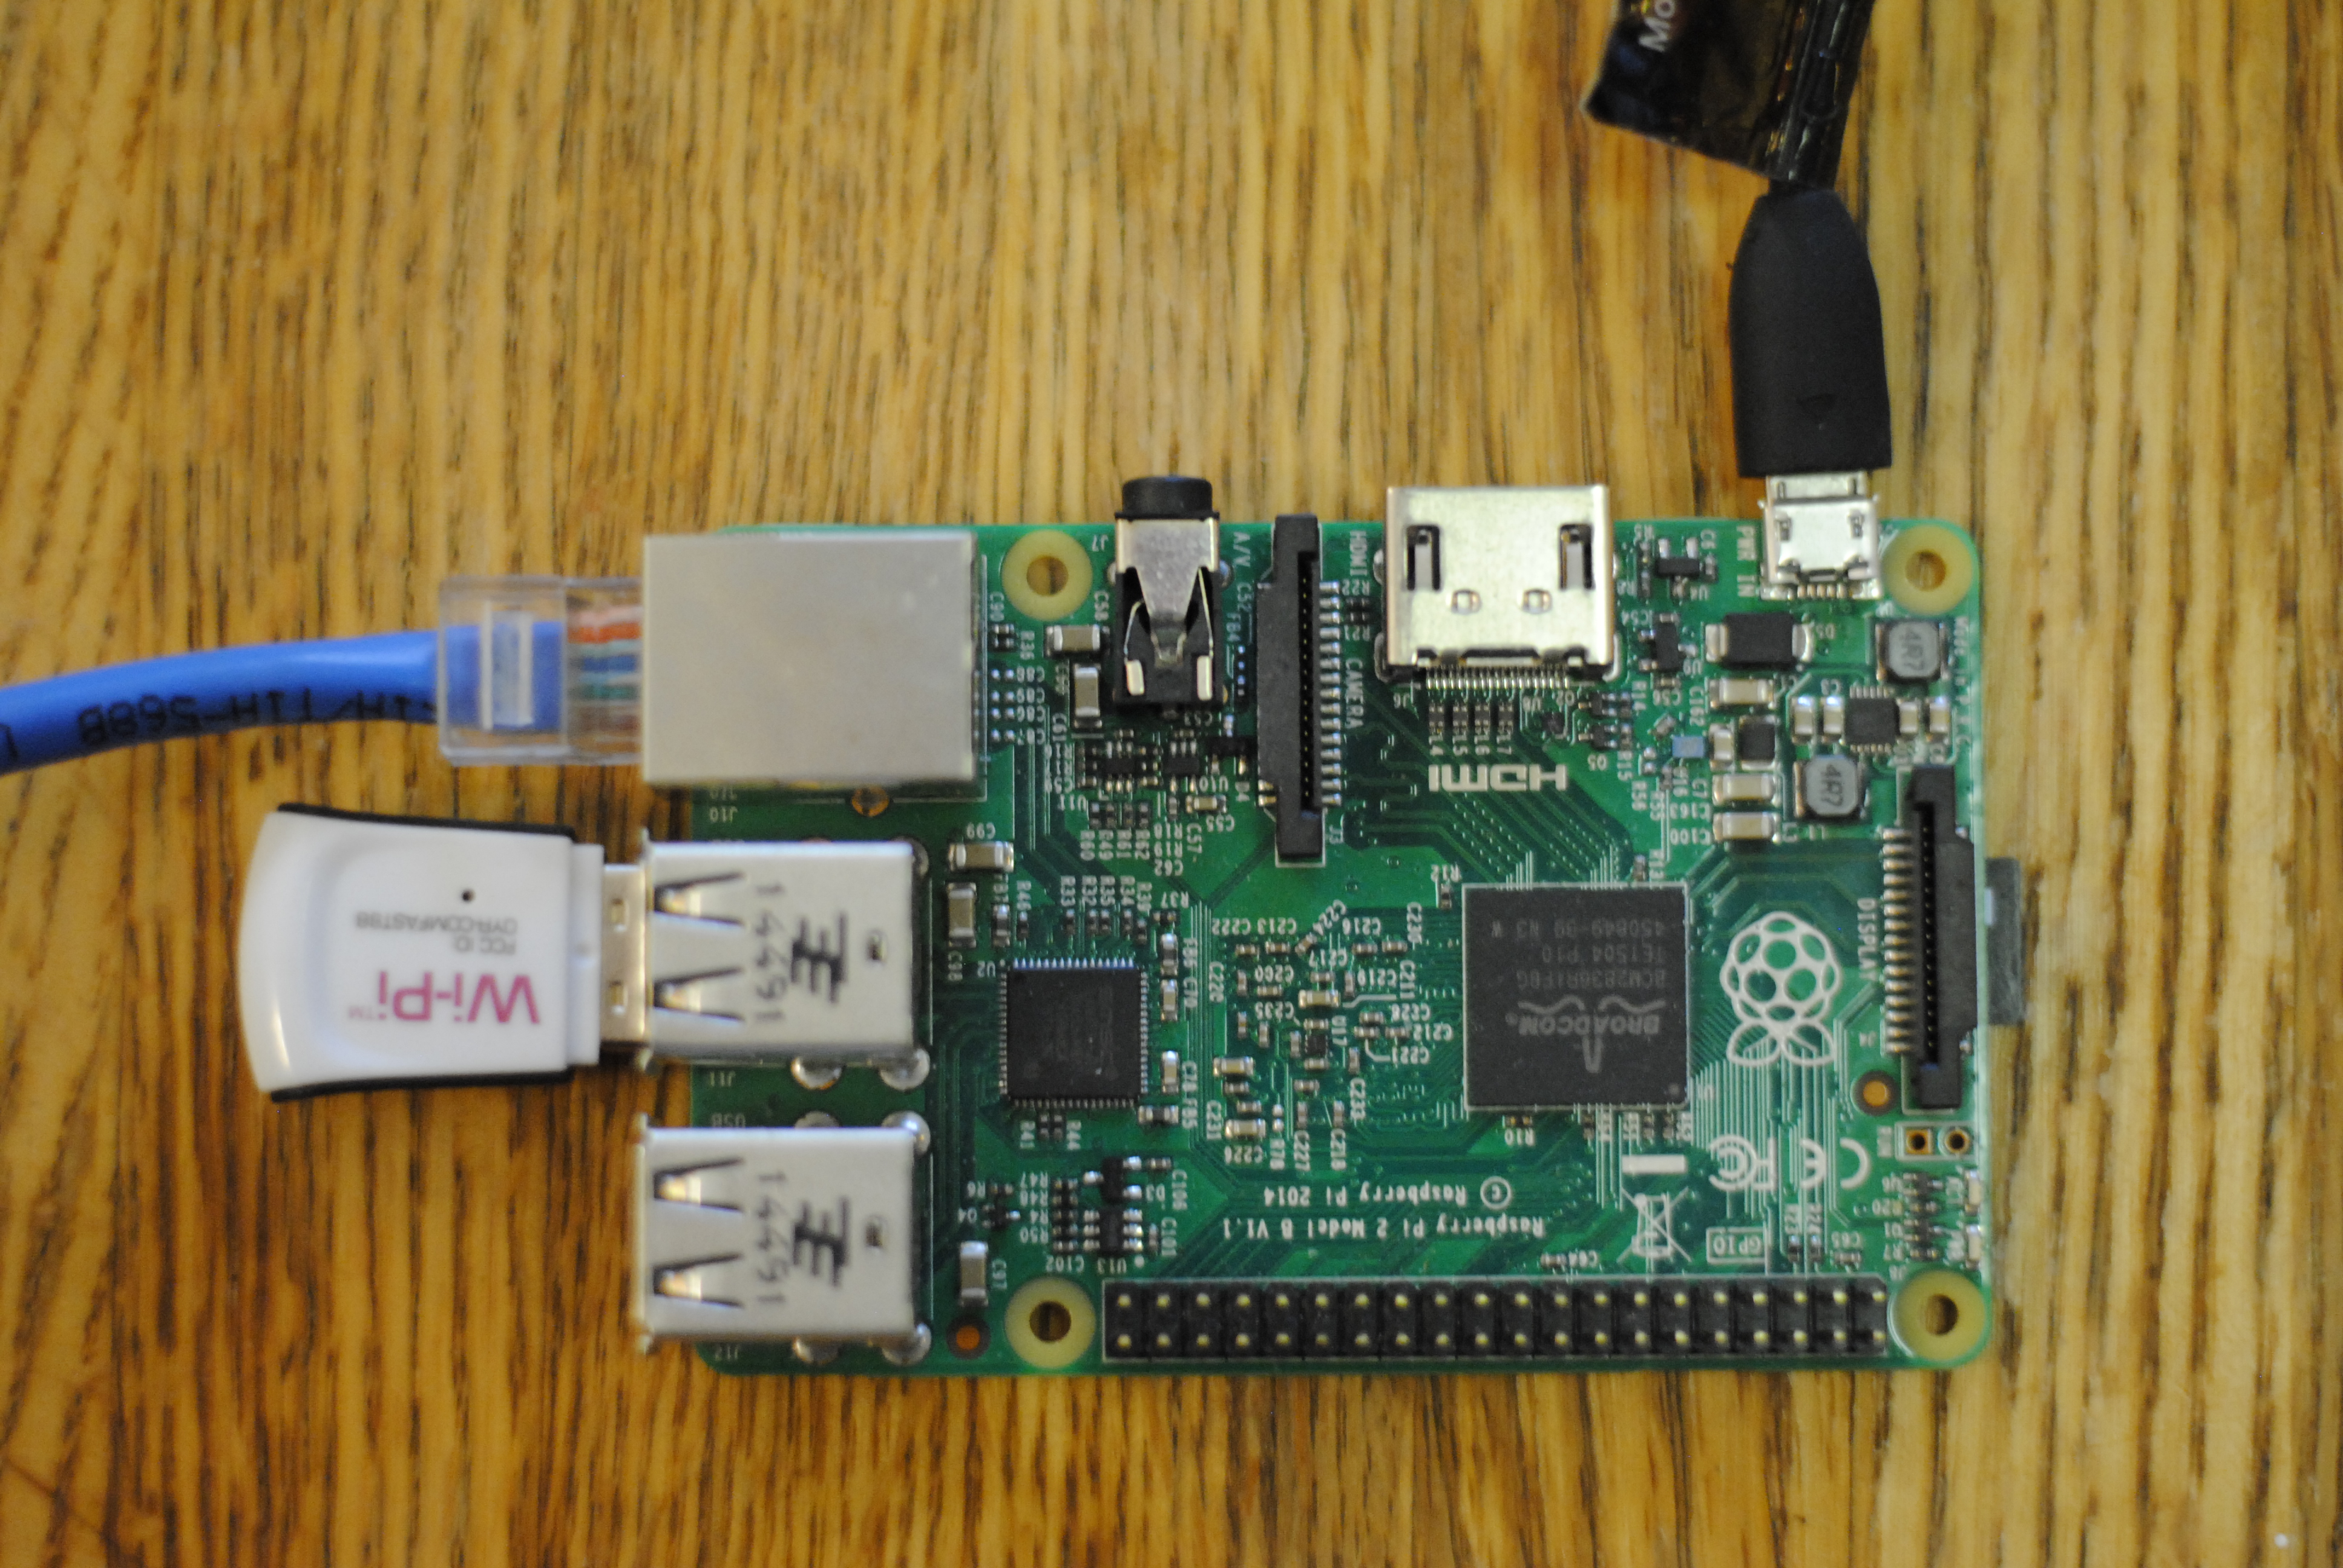
\includegraphics[width=\textwidth, keepaspectratio=true]{Graphics/Controller.JPG}
	\caption{BatSignal Control Node}
\end{figure}

\subsection{Sensor Node}
\begin{figure}[H]
	\centering
		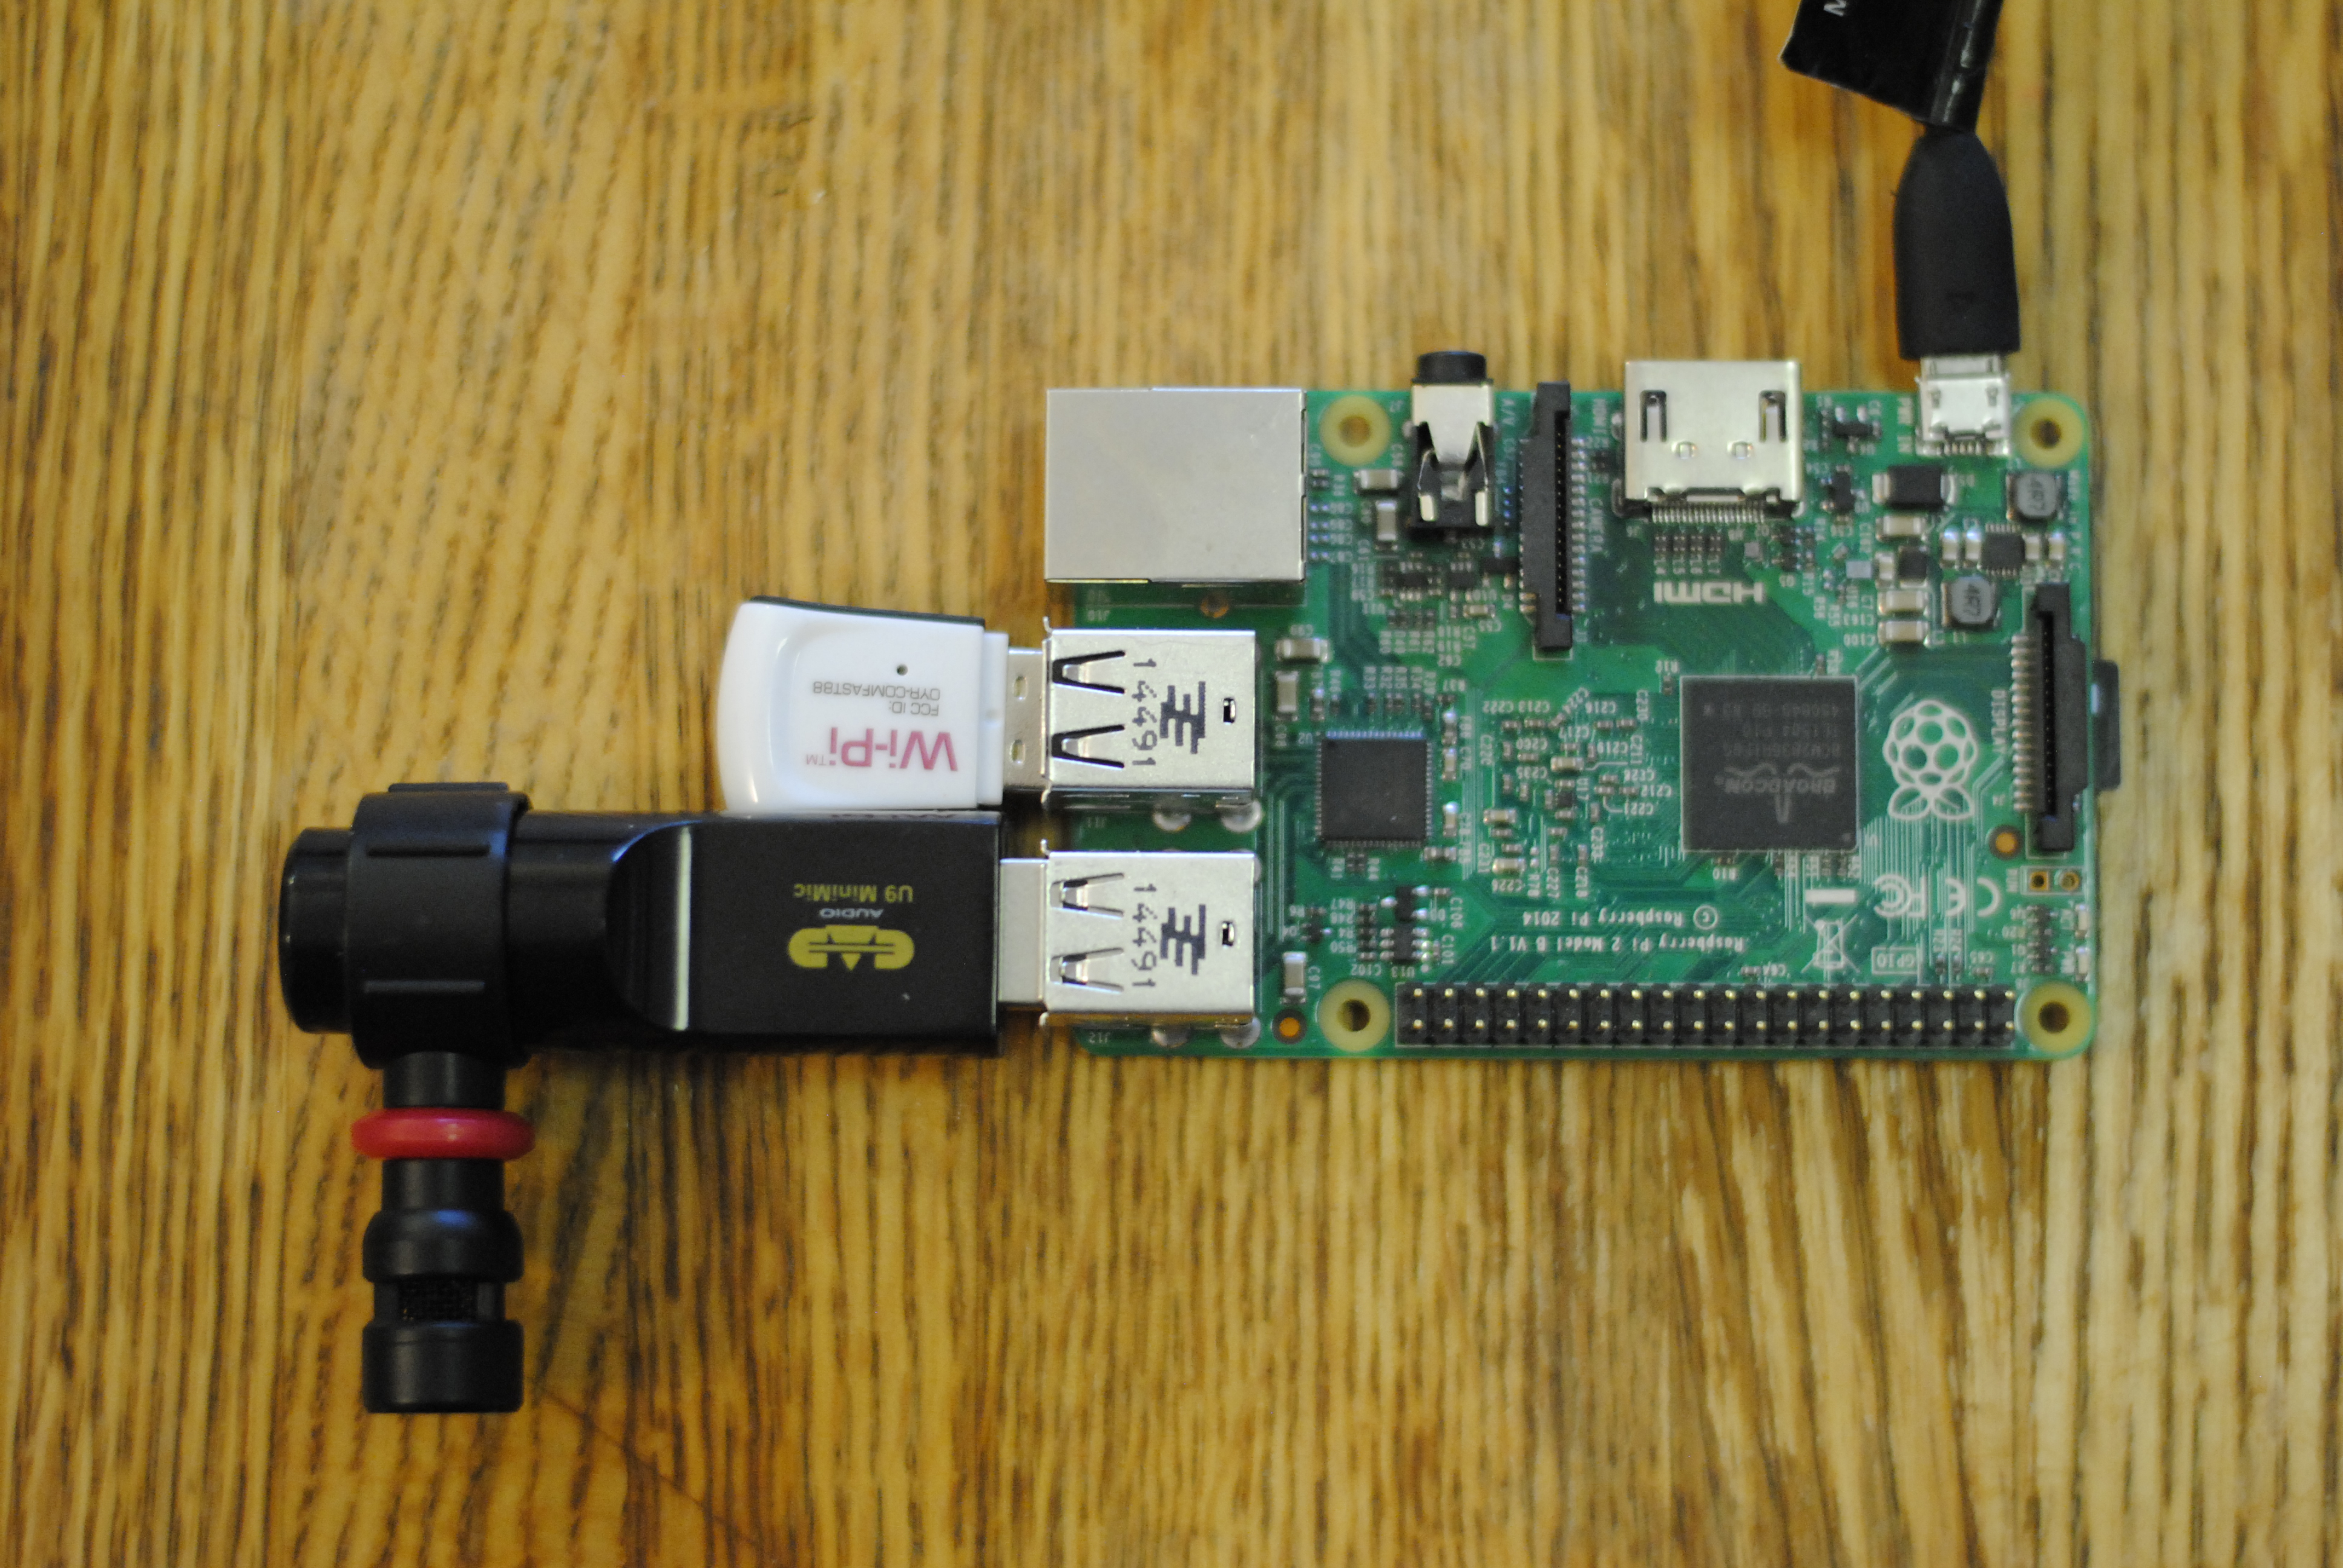
\includegraphics[width=\textwidth, keepaspectratio=true]{Graphics/Sensor.JPG}
	\caption{BatSignal Sensor Node}
\end{figure}

\section{Progress}
\begin{center}
\begin{tabularx}{\textwidth}{ | X | l | }
	\hline
	Task & Status \\
	\hline
	Python sensor module 				& Complete 		\\
	Python control module 				& Complete 		\\
	Administration web console 			& In Progress 	\\
	Installation scripts				& Complete		\\
	BATMAN Gateway configuration		& Complete		\\
	BATMAN Node configuration			& Complete		\\
	\hline
\end{tabularx}
\end{center}

\section{Future Development}
\begin{list}{-}{}
	\item{Replace PyAudio library}\\
	\phantom{00}\textit{PyAudio has internal threading issues that causes intermittent deadlock.}
	\item{Replace speech\_{}recognition}\\
	\phantom{00}\textit{Google's text-to-speech API doesn't support multiple speakers, and is trained on Google search data leading to incorrect translations.}
	\item{Replace microphones}\\
	\phantom{00}\textit{Audio pickup range is too short, audio quality is poor, and the microphone picks up system noise.}
	\item{Explore alternatives to the Raspberry Pi}\\
	\phantom{00}\textit{Raspberry Pi devices have poor audio quality due to electrical noise within the system.}
	\item{Migrate code base to C}\\
	\phantom{00}\textit{The desire is to have an extensible framework which is also capable of handling a higher number of requests within the network. Also, to integrate more sophisticated keyword detection using natural language processing.}	
	\item{DHCP within the BATMAN mesh}\\
	\phantom{00}\textit{Allow for dynamic allocation of addresses within the mesh network subnet to better facilitate ad-hoc connections and network scalability.}
	\item{Integrate Alfred with BATMAN}\\
	\phantom{00}\textit{Alfred extends the functionality of BATMAN and would allow for live modeling of the network traffic. Also allows for further extensibility (ie: sharing geo-location data and topological mapping).}
	\item{Network security}\\
	\phantom{00}\textit{Messages are unencrypted, SSID is openly broadcast, no passkey is necessary to connect to the BATMAN mesh network. Devices are only configured as necessary, security is not built in. Devices have no authentication. The username and password used for email dispatch is hard-coded in the open-source code base. Further concerns must also be identified and addressed.}
	\item{Alternative power solution}\\
	\phantom{00}\textit{As it stands the devices are required to be wired directly into an outlet to receive continual power. Alternative solutions for powering the device, including battery backups, would improve system reliability.}
\end{list}

This project is under continuing development and future development items may be addressed or updated since the publication of this document. Please consult the open-source Github repository \texttt{https://github.com/YoungB2/BatSignal} for Issues tracking development tasks. The release published at the time of this document's writing is tagged as \texttt{0.1-submission}. 

\end{document}